% =============================================================================
% cover-farbschema.tex – Cover für Farbschema-Dokumentation
% =============================================================================
% Kompilieren: xelatex cover-farbschema.tex
% Erzeugt: cover-farbschema.pdf (für \coverimage in farbschema.tex)
% =============================================================================
\documentclass[tikz,border=0pt]{standalone}

% -----------------------------------------------------------------------------
% SCHRIFTEN (identisch mit techdoc.cls)
% -----------------------------------------------------------------------------
\usepackage{fontspec}
\defaultfontfeatures{Ligatures=TeX}

\setmainfont{TeX Gyre Pagella}
\setsansfont{TeX Gyre Heros}
\setmonofont[Scale=0.85]{TeX Gyre Cursor}

% -----------------------------------------------------------------------------
% FARBEN (identisch mit techdoc.cls)
% -----------------------------------------------------------------------------
\usepackage{xcolor}

% Primärfarben
\definecolor{ArduinoTeal}{HTML}{00979D}
\definecolor{ArduinoDark}{HTML}{005C5F}
\definecolor{RaspberryRed}{HTML}{C51A4A}
\definecolor{RaspberryPurple}{HTML}{75264A}

% Statusfarben
\definecolor{SuccessGreen}{HTML}{75A928}
\definecolor{WarningOrange}{HTML}{D97706}

% Hintergründe
\definecolor{GitHubDark}{HTML}{0D1117}
\definecolor{SlateDark}{HTML}{1E2933}
\definecolor{SlateMedium}{HTML}{2D3A45}

% Text
\definecolor{LightText}{HTML}{E6EDF3}
\definecolor{MutedText}{HTML}{4A5568}

% Signalfarben
\definecolor{SignalData}{HTML}{51CF66}
\definecolor{SignalClock}{HTML}{FFD43B}
\definecolor{SignalLatch}{HTML}{4DABF7}

% Box-Farben
\definecolor{InfoBoxBg}{HTML}{E6F5FA}
\definecolor{WarnBoxBg}{HTML}{FFF7ED}

% -----------------------------------------------------------------------------
% TIKZ-BIBLIOTHEKEN
% -----------------------------------------------------------------------------
\usetikzlibrary{shapes, arrows.meta, positioning, calc}

% -----------------------------------------------------------------------------
% DOKUMENT
% -----------------------------------------------------------------------------
\begin{document}
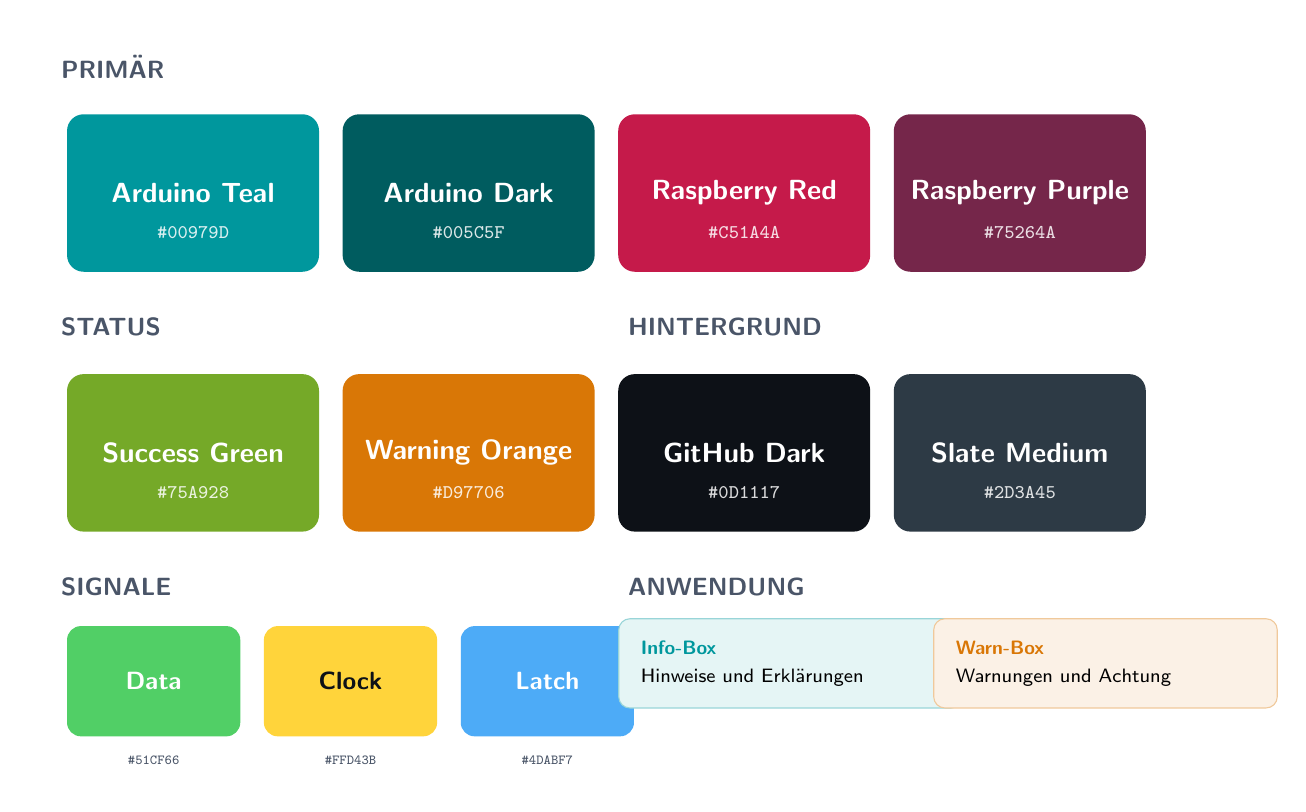
\begin{tikzpicture}[
  % Großer Farbblock mit Hex-Code innen
  colorblock/.style={
    minimum width=3.2cm,
    minimum height=2.0cm,
    rounded corners=6pt,
    font=\sffamily\bfseries,
    text=white,
    inner sep=0pt
  },
  % Kleiner Farbblock für Signale
  smallblock/.style={
    minimum width=2.2cm,
    minimum height=1.4cm,
    rounded corners=5pt,
    font=\sffamily\bfseries\small,
    text=white,
    inner sep=0pt
  },
  % Section-Label
  seclbl/.style={
    font=\sffamily\bfseries\small,
    color=MutedText
  },
  % Infobox
  infobox/.style={
    draw=#1!40,
    fill=#1!10,
    rounded corners=4pt,
    font=\sffamily\scriptsize,
    text width=3.8cm,
    align=left,
    inner sep=8pt
  },
  infobox/.default=ArduinoTeal
]

% =============================================================================
% HINTERGRUND
% =============================================================================
\fill[white] (-0.3,-0.3) rectangle (14.3,9.3);

% =============================================================================
% PRIMÄRFARBEN
% =============================================================================
\node[seclbl, anchor=west] at (0,8.8) {PRIMÄR};

% Arduino Teal
\node[colorblock, fill=ArduinoTeal] (teal) at (1.8,7.2) {};
\node[font=\sffamily\bfseries, text=white] at (teal.center) {Arduino Teal};
\node[font=\ttfamily\scriptsize, text=white, opacity=0.85] at ([yshift=-0.5cm]teal.center) {\#00979D};

% Arduino Dark
\node[colorblock, fill=ArduinoDark] (dark) at (5.3,7.2) {};
\node[font=\sffamily\bfseries, text=white] at (dark.center) {Arduino Dark};
\node[font=\ttfamily\scriptsize, text=white, opacity=0.85] at ([yshift=-0.5cm]dark.center) {\#005C5F};

% Raspberry Red
\node[colorblock, fill=RaspberryRed] (red) at (8.8,7.2) {};
\node[font=\sffamily\bfseries, text=white] at (red.center) {Raspberry Red};
\node[font=\ttfamily\scriptsize, text=white, opacity=0.85] at ([yshift=-0.5cm]red.center) {\#C51A4A};

% Raspberry Purple
\node[colorblock, fill=RaspberryPurple] (purple) at (12.3,7.2) {};
\node[font=\sffamily\bfseries, text=white] at (purple.center) {Raspberry Purple};
\node[font=\ttfamily\scriptsize, text=white, opacity=0.85] at ([yshift=-0.5cm]purple.center) {\#75264A};

% =============================================================================
% STATUS (links)
% =============================================================================
\node[seclbl, anchor=west] at (0,5.5) {STATUS};

% Success Green
\node[colorblock, fill=SuccessGreen] (green) at (1.8,3.9) {};
\node[font=\sffamily\bfseries, text=white] at (green.center) {Success Green};
\node[font=\ttfamily\scriptsize, text=white, opacity=0.85] at ([yshift=-0.5cm]green.center) {\#75A928};

% Warning Orange
\node[colorblock, fill=WarningOrange] (orange) at (5.3,3.9) {};
\node[font=\sffamily\bfseries, text=white] at (orange.center) {Warning Orange};
\node[font=\ttfamily\scriptsize, text=white, opacity=0.85] at ([yshift=-0.5cm]orange.center) {\#D97706};

% =============================================================================
% HINTERGRUND (rechts)
% =============================================================================
\node[seclbl, anchor=west] at (7.2,5.5) {HINTERGRUND};

% GitHub Dark
\node[colorblock, fill=GitHubDark] (gh) at (8.8,3.9) {};
\node[font=\sffamily\bfseries, text=white] at (gh.center) {GitHub Dark};
\node[font=\ttfamily\scriptsize, text=white, opacity=0.85] at ([yshift=-0.5cm]gh.center) {\#0D1117};

% Slate Medium
\node[colorblock, fill=SlateMedium] (slate) at (12.3,3.9) {};
\node[font=\sffamily\bfseries, text=white] at (slate.center) {Slate Medium};
\node[font=\ttfamily\scriptsize, text=white, opacity=0.85] at ([yshift=-0.5cm]slate.center) {\#2D3A45};

% =============================================================================
% SIGNALE (links unten)
% =============================================================================
\node[seclbl, anchor=west] at (0,2.2) {SIGNALE};

% Data
\node[smallblock, fill=SignalData] (data) at (1.3,1.0) {};
\node[font=\sffamily\bfseries\small, text=white] at (data.center) {Data};
\node[font=\ttfamily\tiny, text=MutedText] at ([yshift=-1.0cm]data.center) {\#51CF66};

% Clock
\node[smallblock, fill=SignalClock] (clock) at (3.8,1.0) {};
\node[font=\sffamily\bfseries\small, text=GitHubDark] at (clock.center) {Clock};
\node[font=\ttfamily\tiny, text=MutedText] at ([yshift=-1.0cm]clock.center) {\#FFD43B};

% Latch
\node[smallblock, fill=SignalLatch] (latch) at (6.3,1.0) {};
\node[font=\sffamily\bfseries\small, text=white] at (latch.center) {Latch};
\node[font=\ttfamily\tiny, text=MutedText] at ([yshift=-1.0cm]latch.center) {\#4DABF7};

% =============================================================================
% ANWENDUNG (rechts unten)
% =============================================================================
\node[seclbl, anchor=west] at (7.2,2.2) {ANWENDUNG};

% Info-Box Preview
\node[infobox=ArduinoTeal, anchor=north west] (infobox) at (7.2,1.8) {
  \textcolor{ArduinoTeal}{\textbf{Info-Box}}\\[2pt]
  Hinweise und Erklärungen
};

% Warn-Box Preview
\node[infobox=WarningOrange, anchor=north west] at (11.2,1.8) {
  \textcolor{WarningOrange}{\textbf{Warn-Box}}\\[2pt]
  Warnungen und Achtung
};

\end{tikzpicture}
\end{document}
